\documentclass[]{beamer}
\usepackage{xmpmulti}
\setbeamertemplate{navigation symbols}{}
\setbeamertemplate{itemize items}[ball]
\usepackage{animate}
\usetheme{CambridgeUS}
\usepackage[style=ieee]{biblatex}
\usecolortheme{seahorse}
\usepackage[]{algorithm2e}
\bibliography{references}
\beamersetuncovermixins{\opaqueness<1>{25}}{\opaqueness<2->{15}}

\usepackage{amssymb}
\usepackage{amsmath}
\usepackage{mathrsfs}
\usepackage{bbm}

\usepackage{subfig}

\newcommand{\vect}{\boldsymbol}

\usepackage[absolute,overlay]{textpos}
\newenvironment{reference}[2]
    {\begin{textblock*}{\textwidth}(#1,#2)
        \footnotesize\it\bgroup\color{red!50!black}}
    {\egroup\end{textblock*}}


\begin{document}

\title{Resonant Driving Induced Ferromagnetism \\ in Fermi Hubbard Model}
\author{Ning Sun}
\institute{Tsinghua University}
\date{\today}

\begin{frame}

    {
        \titlepage
    }
    
    \begin{reference}{4mm}{85mm}
        NS, Pengfei Zhang, Hui Zhai, arXiv:1808.03966v2.
    \end{reference}
\end{frame}


\section{General Overview}
\small
\begin{frame}\frametitle{Introduction}
\begin{block}{ETH group experiment: periodically shaking honeycomb lattice}
\begin{figure}
    \centering
    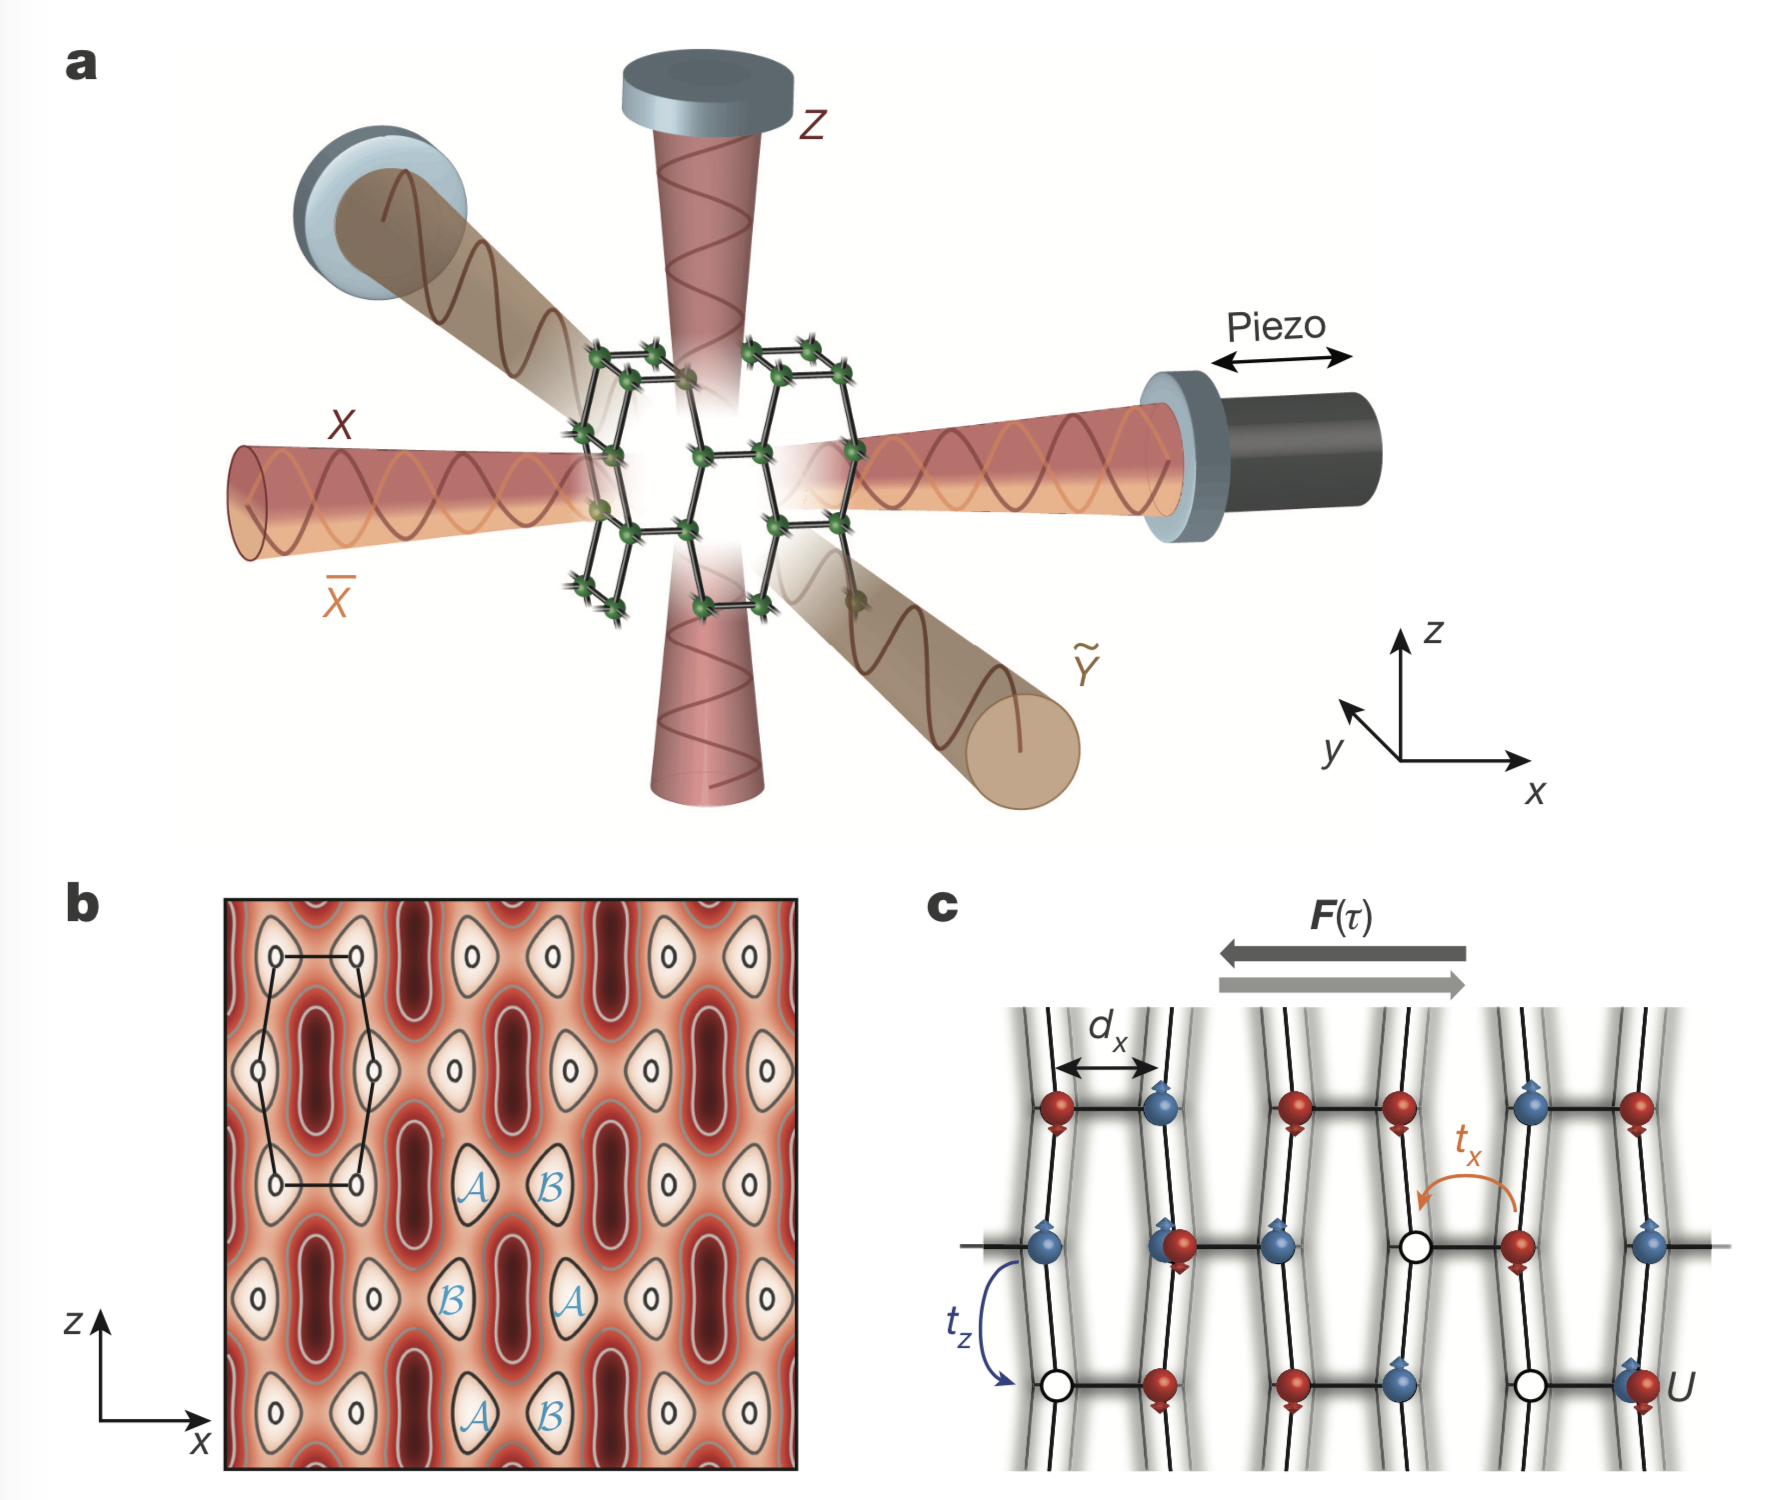
\includegraphics[width=0.5\columnwidth]{figs/eth.png}
\end{figure}
\footnote{ETH group, Enhancement and sign change of magnetic correlations in a 
    driven quantum many-body system, Nature 553, 481-485 (2018).}
\end{block}

\end{frame}


\section{Model}

\subsection{Periodically driven Fermi Hubbard model}
\begin{frame}\frametitle{Periodically driven Fermi Hubbard model}
\pause
\begin{block}{Time-dependent Hamiltonian}
% \small
\begin{align*} % \label{eq:H}
    \hat{H}(t) =& -J \sum_{\substack{\langle i,j\rangle \\ 
    \sigma = \uparrow,\downarrow}} e^{i\mathbf{d_{ij}}\cdot \mathbf{A}(t)/\hbar}
    \hat{c}_{i\sigma}^{\dagger}\hat{c}_{j\sigma}
    +U\sum_{i}\left(\hat{n}_{i\uparrow}-\frac{1}{2}\right)
    \left(\hat{n}_{i\downarrow}-\frac{1}{2}\right)
\end{align*}
\end{block}
\begin{block}{}
\begin{figure}[!htb]
    \centering
    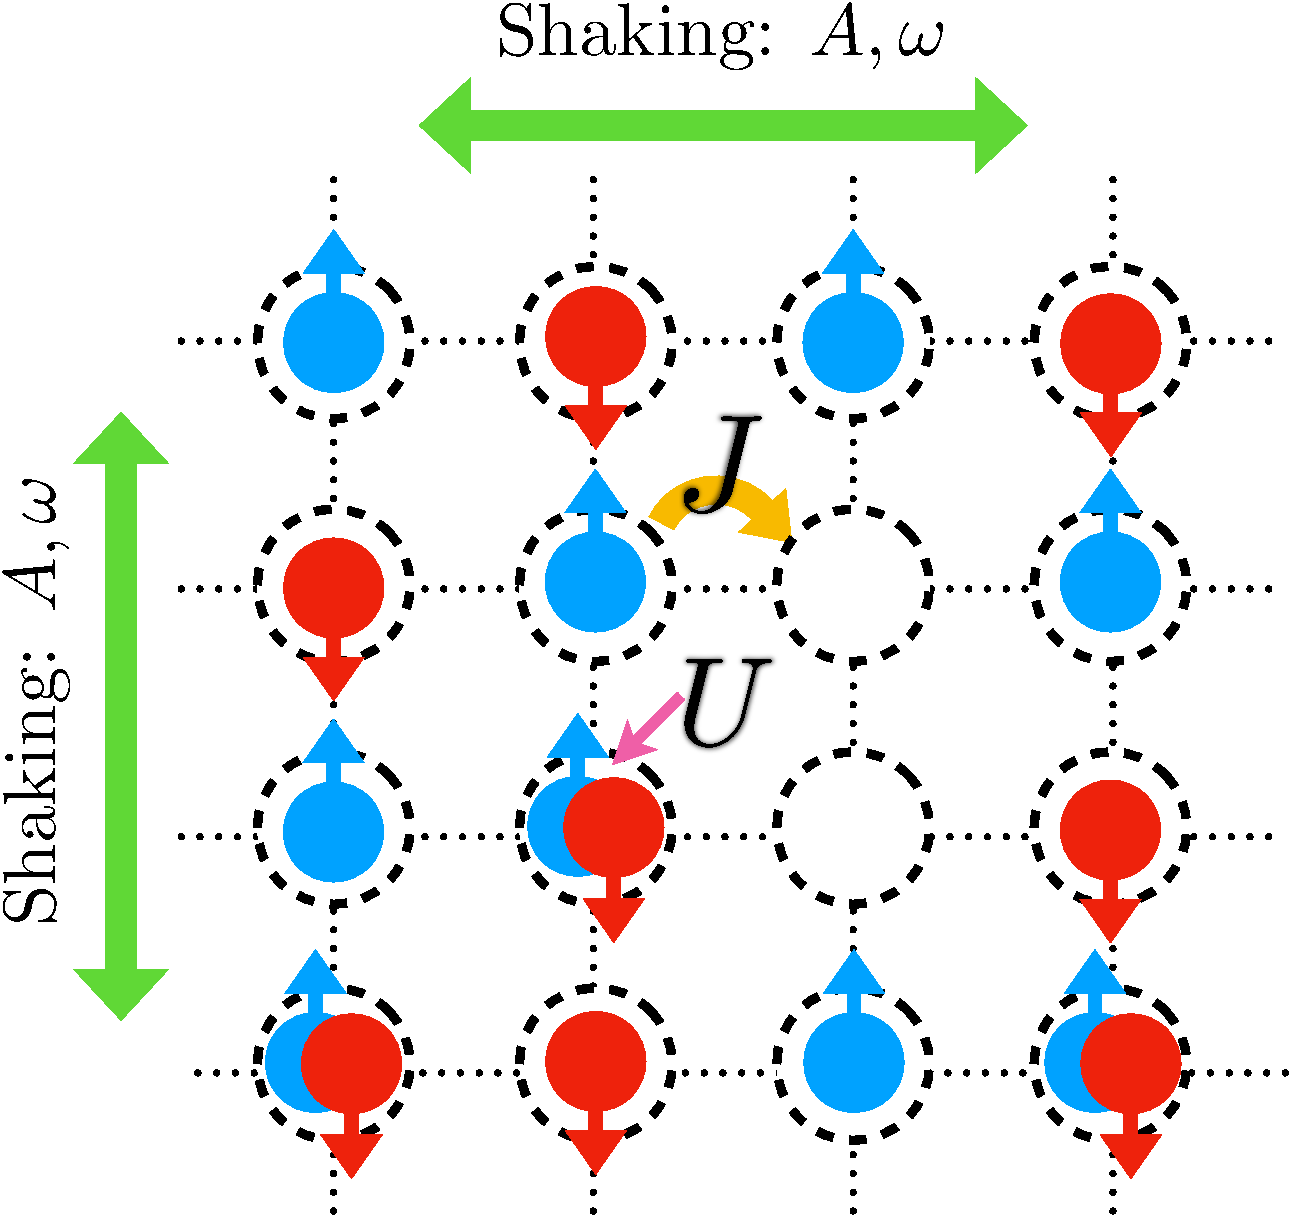
\includegraphics[width=0.4\columnwidth]{figs/schematic.pdf}
\end{figure}
\end{block}
\end{frame}

\begin{frame}
\frametitle{High-frequency expansion}
\pause
\begin{block}{far-off resonance and high frequency}
\begin{minipage}{.3\columnwidth}
\pause
    \only<1-|handout:0>{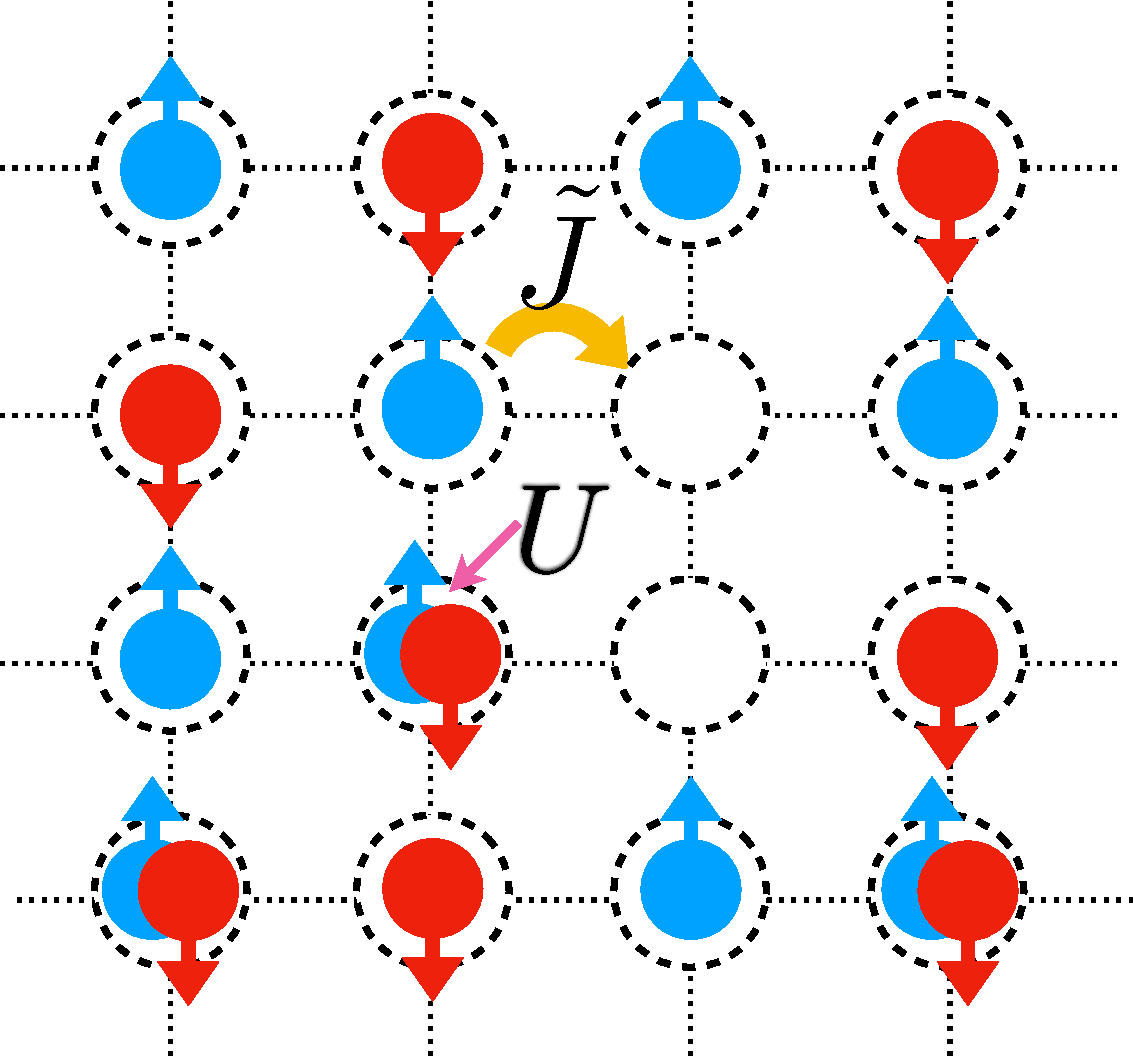
\includegraphics[width=.99\columnwidth]{figs/heff.pdf}}
\end{minipage}
\begin{minipage}{.65\columnwidth}
\begin{figure}[!htb]
\centering
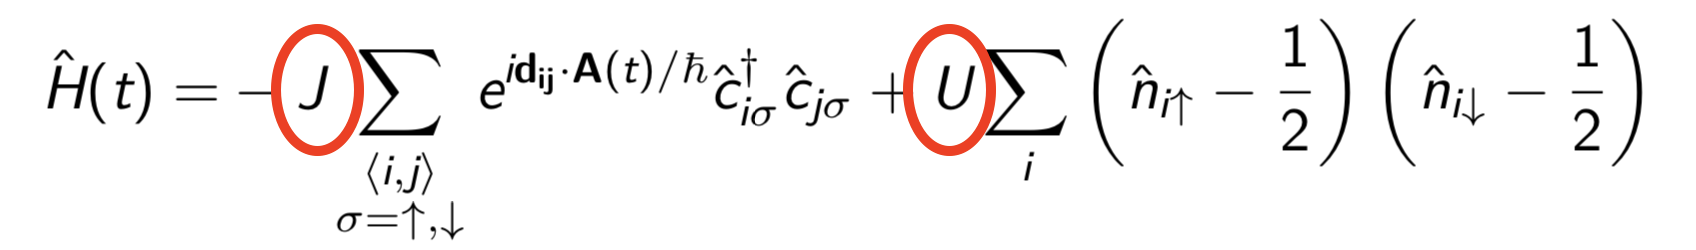
\includegraphics[width=1.08\columnwidth]{figs/Ht.png}
\end{figure}
\begin{align*}
    \dfrac{1}{T}\int_0^T e^{i\mathbf{d_{ij}}\cdot \mathbf{A}(t)/\hbar} dt 
    = \mathcal{B}_0(mA\omega d/\hbar)
\end{align*}
\begin{align*}
    J \rightarrow \tilde{J} = J\mathcal{B}_0(\mathcal{A}), 
    \quad \text{with} \; \mathcal{A} = mA\omega d/\hbar
\end{align*}
\end{minipage}
\pause
\end{block}
\begin{block}{near resonance}
\vspace{-3ex}
\begin{align*}
    U \sim l\hbar\omega \quad \rightarrow \quad \tilde{U} = U - l\hbar\omega
\end{align*}
\vspace{-5ex}
\begin{align*}
    \tilde{U} \sim J \ll \omega
\end{align*}
\end{block}
\end{frame}

\begin{frame} % \frametitle{Periodically driven Fermi Hubbard model}
\pause
\footnotesize
\begin{block}{Unitary transformation}
\vspace{-3ex}
\begin{align*}
    \hat{R}(t)=\exp(i\sum_{j}l\omega t\hat{n}_{j\uparrow}\hat{n}_{j\downarrow})
\end{align*}
\vspace{-5ex}
\begin{align*}
    \tilde{\mathbf{A}}_{ij,\sigma}(t)&=\mathbf{A}(t)
        -\frac{l\omega t}{d^2} \mathbf{d_{ij}}
        ((1-\hat n_{i\bar\sigma})\hat n_{j\bar\sigma}
         -(1-\hat n_{j\bar\sigma})\hat n_{i\bar\sigma}))
\end{align*}
\end{block}
\pause
\begin{block}{Effective static Hamiltonian}
\begin{align*}
    \hat{H}_{\text{eff}} = \sum_{\langle i,j\rangle, \sigma} 
        -\hat{J}^{\langle ij\rangle}_{\text{eff},\sigma}
        \hat{c}_{i\sigma}^{\dagger}\hat{c}_{j\sigma} 
    + \tilde{U}\sum_{i}\left(\hat{n}_{i\uparrow}-\frac{1}{2}\right)
        \left(\hat{n}_{i\downarrow}-\frac{1}{2}\right).  % \label{Heff}
\end{align*}
\vspace{-3ex}
\begin{align*}
    \hat{J}^{\langle ij\rangle}_{\text{eff},\sigma}=
        J_0\hat{a}_{ij\bar{\sigma}}+J_1\hat{b}_{ij\bar{\sigma}} , 
    \qquad
    \tilde{U} = U - l\hbar\omega
\end{align*}
\vspace{-3ex}
\begin{align*}
    \hat{a}_{ij\sigma} &= (1-\hat{n}_{i\sigma})(1-\hat{n}_{j\sigma}) 
        + \hat{n}_{i\sigma}\hat{n}_{j\sigma},\\
	\hat{b}_{ij\sigma} &= (-1)^l(1-\hat{n}_{i\sigma})\hat{n}_{j\sigma} 
        + \hat{n}_{i\sigma}(1-\hat{n}_{j\sigma}).
\end{align*}
\end{block}
\pause
\begin{block}{Symmetry}
\begin{itemize}
    \item SO(4) symmetry of even $l$
    \item particle-hole symmetry at half filling
\end{itemize}
\end{block}
\end{frame}


\subsection{Mean field atreatment}
\begin{frame}\frametitle{Mean field theory: a path integral approach}
\pause
\vspace{-2ex}
\begin{block}{real-time partition function}
\vspace{-2ex}
\begin{align*}
    \mathcal{Z}=&\int \mathcal D\psi D\bar\psi \exp(i\int dt L)  \\
    L=&\sum_{i,\sigma} i\bar \psi_{i\sigma}\partial_t\psi_{i\sigma}
    +\sum_{\langle i,j\rangle,\sigma}\left(J_0a_{ij\bar{\sigma}}(\bar\psi \psi) 
        + J_1b_{ij\bar{\sigma}}^l(\bar\psi\psi)\right)\bar 
        \psi_{i\sigma}\psi_{j\sigma} \notag 
    - \tilde{U}\sum_{i}\bar\psi_{i\uparrow}\psi_{i\uparrow}
        \bar\psi_{i\downarrow}\psi_{i\downarrow} \  .
\end{align*}
\end{block}
\pause
\vspace{-1ex}
\begin{block}{mean field Hamiltonian}
\vspace{-2ex}
\begin{align*}
	\hat{H} = \sum_{\langle i,j\rangle, \sigma} 
    - \left(J_0a_{ij\bar{\sigma}}(n) 
                + J_1b_{ij\bar{\sigma}}^l(n)\right)
    \hat{\psi}^{\dagger}_{i\sigma}\hat{\psi}_{j\sigma}  
    + \tilde{U}\sum_{i}n_{i\uparrow}n_{i\downarrow}
    +\sum_{i \sigma}\eta_{i\sigma}(n_{i,\sigma}
                -\hat{\psi}^{\dagger}_{i,\sigma}\hat{\psi}_{i,\sigma}) 
\end{align*}
\vspace{-4ex}
\begin{align*}
\hat{a}_{ij\sigma} &= (1-\hat{n}_{i\sigma})(1-\hat{n}_{j\sigma}) 
    + \hat{n}_{i\sigma}\hat{n}_{j\sigma} 
    \rightarrow (1-n_{i\sigma})(1-n_{j\sigma}) + n_{i\sigma}n_{j\sigma}\\
\hat{b}_{ij\sigma} &= (-1)^l(1-\hat{n}_{i\sigma})\hat{n}_{j\sigma} 
    + \hat{n}_{i\sigma}(1-\hat{n}_{j\sigma})
    \rightarrow (-1)^l(1-n_{i\sigma})n_{j\sigma} + n_{i\sigma}(1-n_{j\sigma})
\end{align*}
\end{block}
\pause
\vspace{-1ex}
\begin{block}{order parameters}
\begin{itemize}
    \item CDF/P
    \item SDW(z)
\end{itemize}
\end{block}
\end{frame}


\section{Quantum Phases}

\subsection{Phase Diagram}
\begin{frame}\frametitle{Quantum phases}
\pause
\begin{block}{Mean field phase diagram and order parameters}
\begin{figure}
    \centering
\pause
    \subfloat[Phase diagram]{
        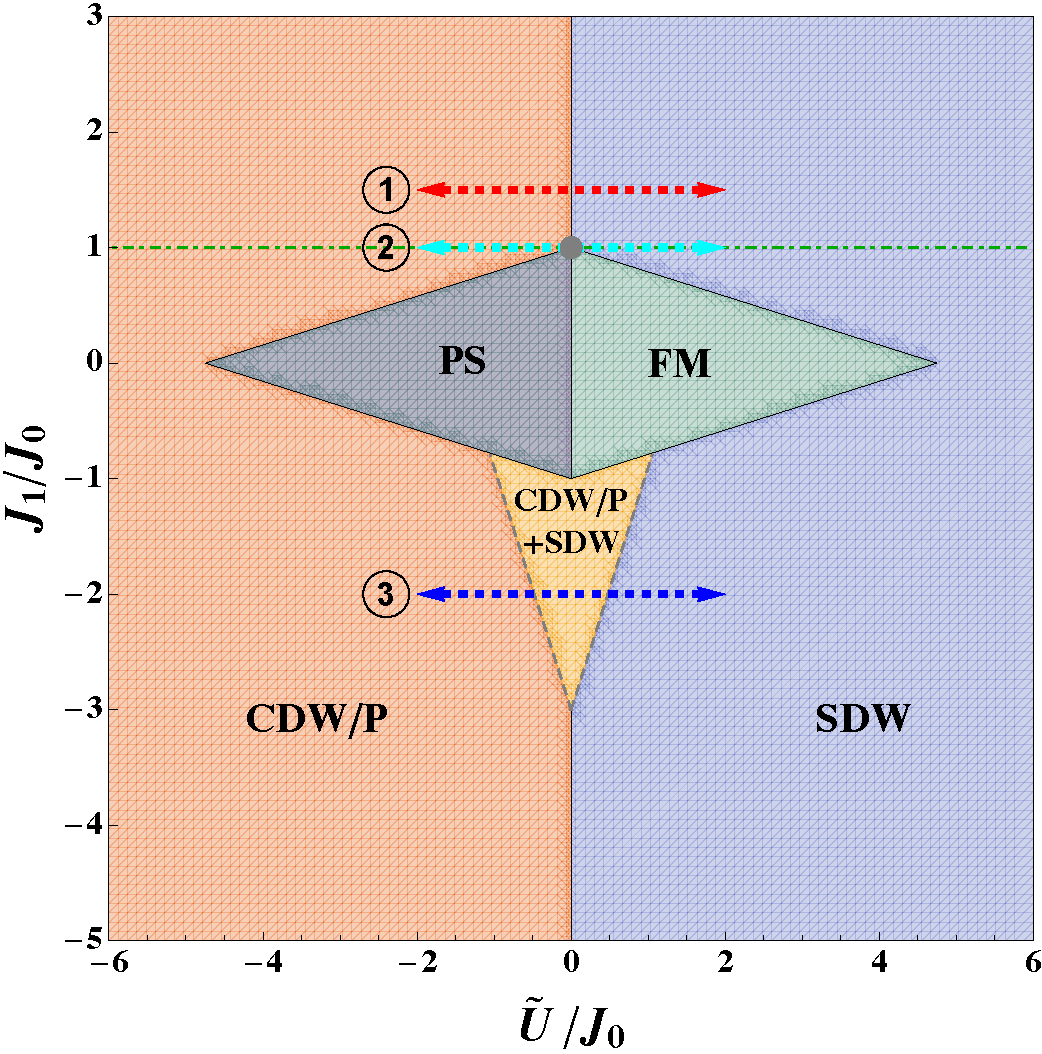
\includegraphics[width=0.4\columnwidth]{figs/Phase_diagram.pdf}
    }
\pause
    \subfloat[Order parameters]{
        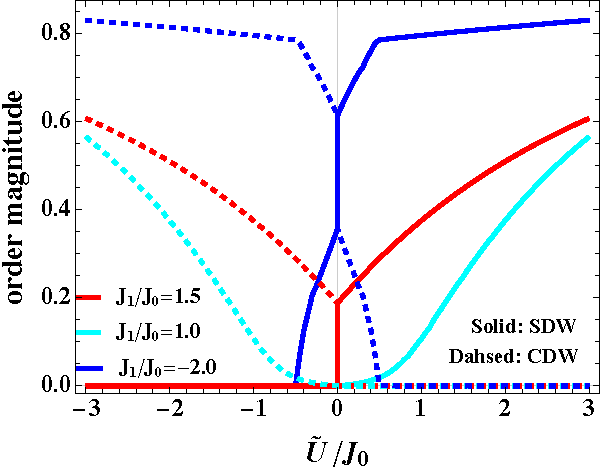
\includegraphics[width=0.4\columnwidth]{figs/order_parameter.pdf}
    }
\end{figure}
\end{block}
\end{frame}

\subsection{Ferromagnetism and phase separation}
\begin{frame} % \frametitle{Ferromagnetism and phase separation}
\begin{block}{Enlarged unit cell calc.}
\begin{figure}[!htb]
    \centering
    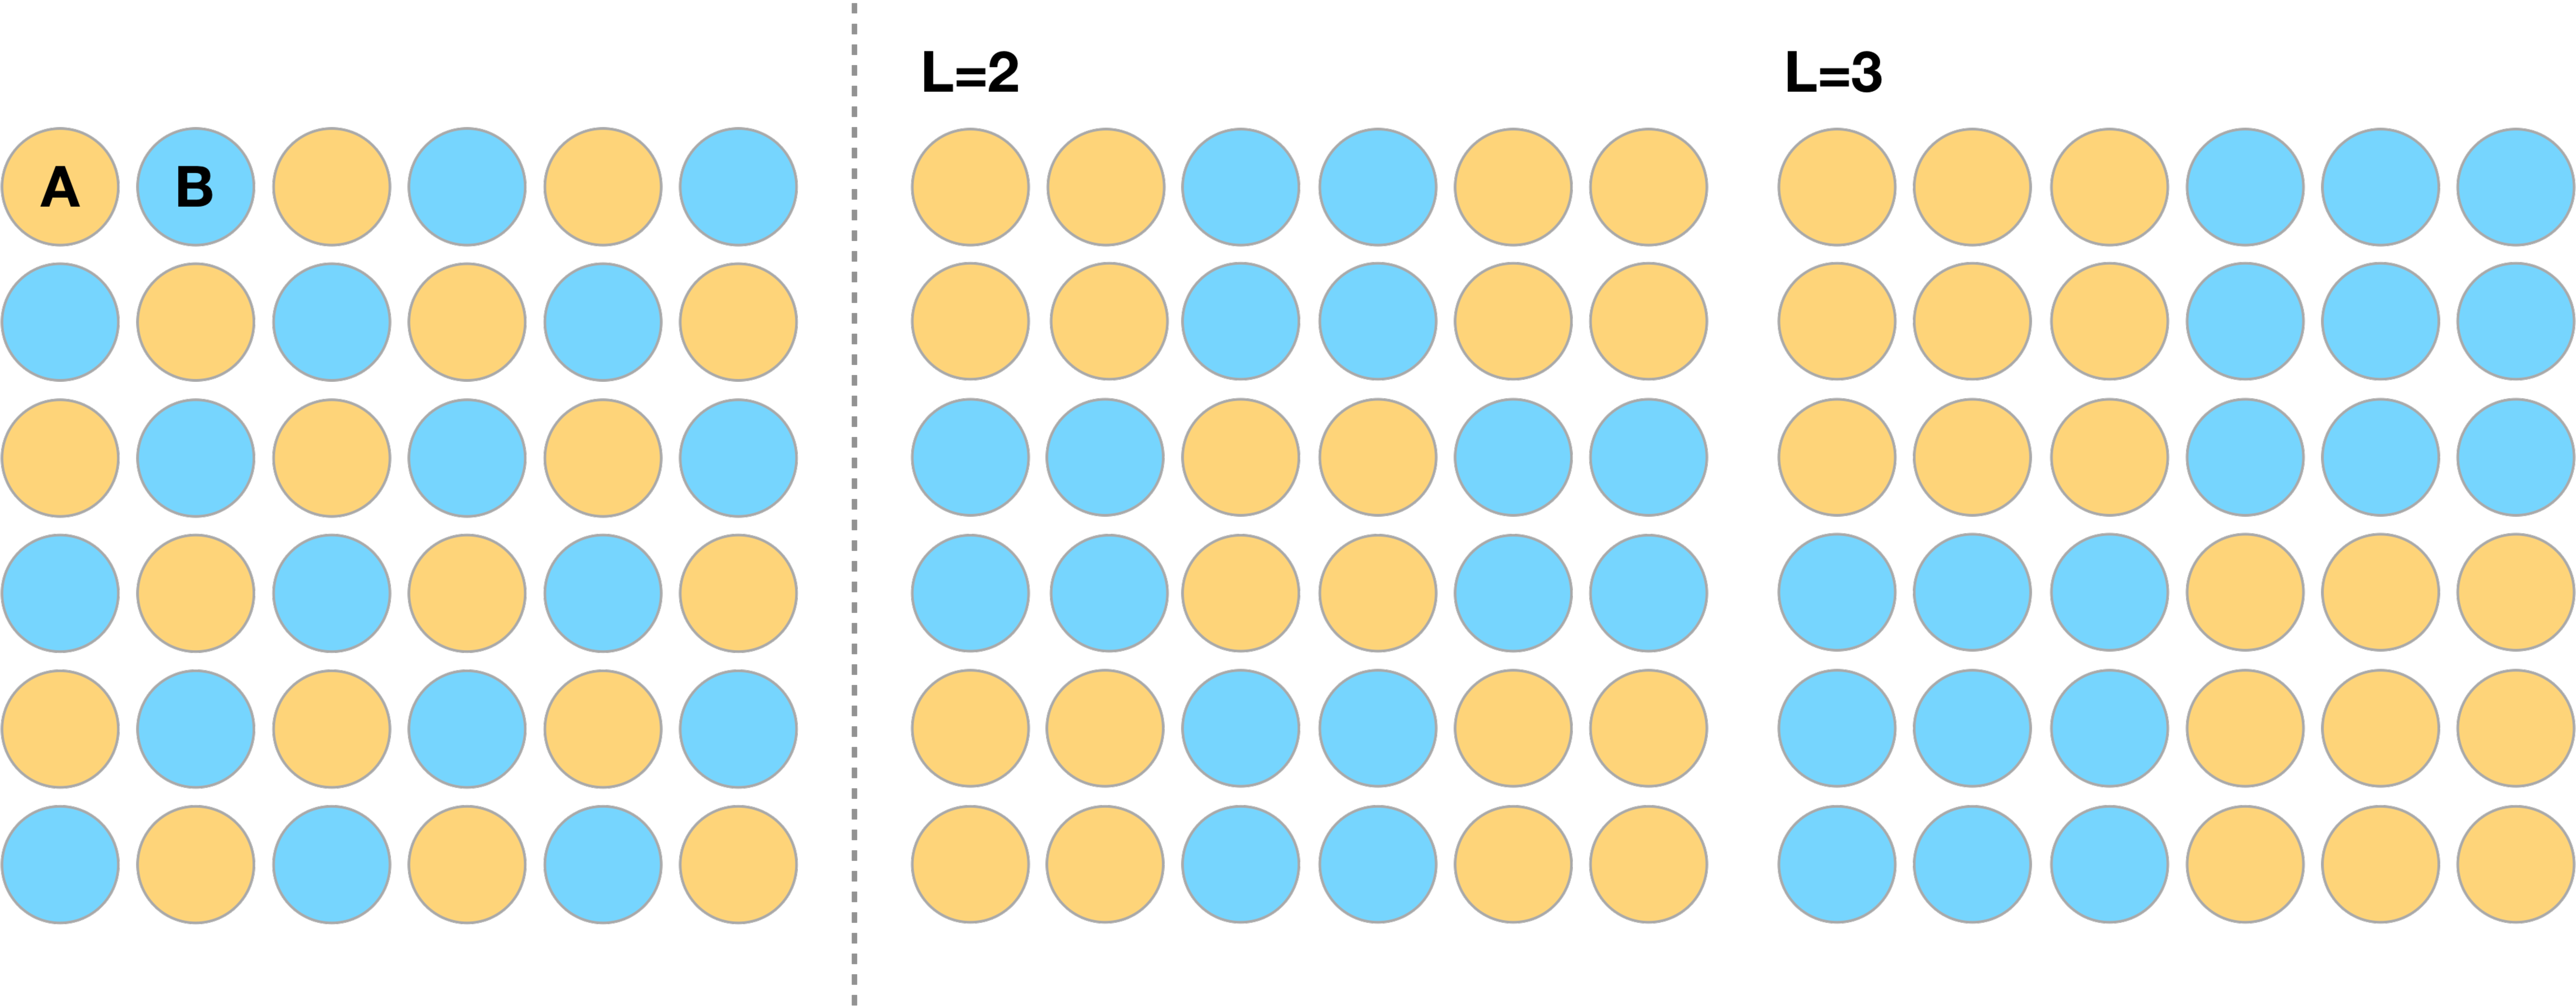
\includegraphics[width=.64\columnwidth]{figs/fig-suppl.pdf}
\end{figure}
\pause
\end{block}
\begin{block}{ground state energy}
\begin{figure}
    \centering
    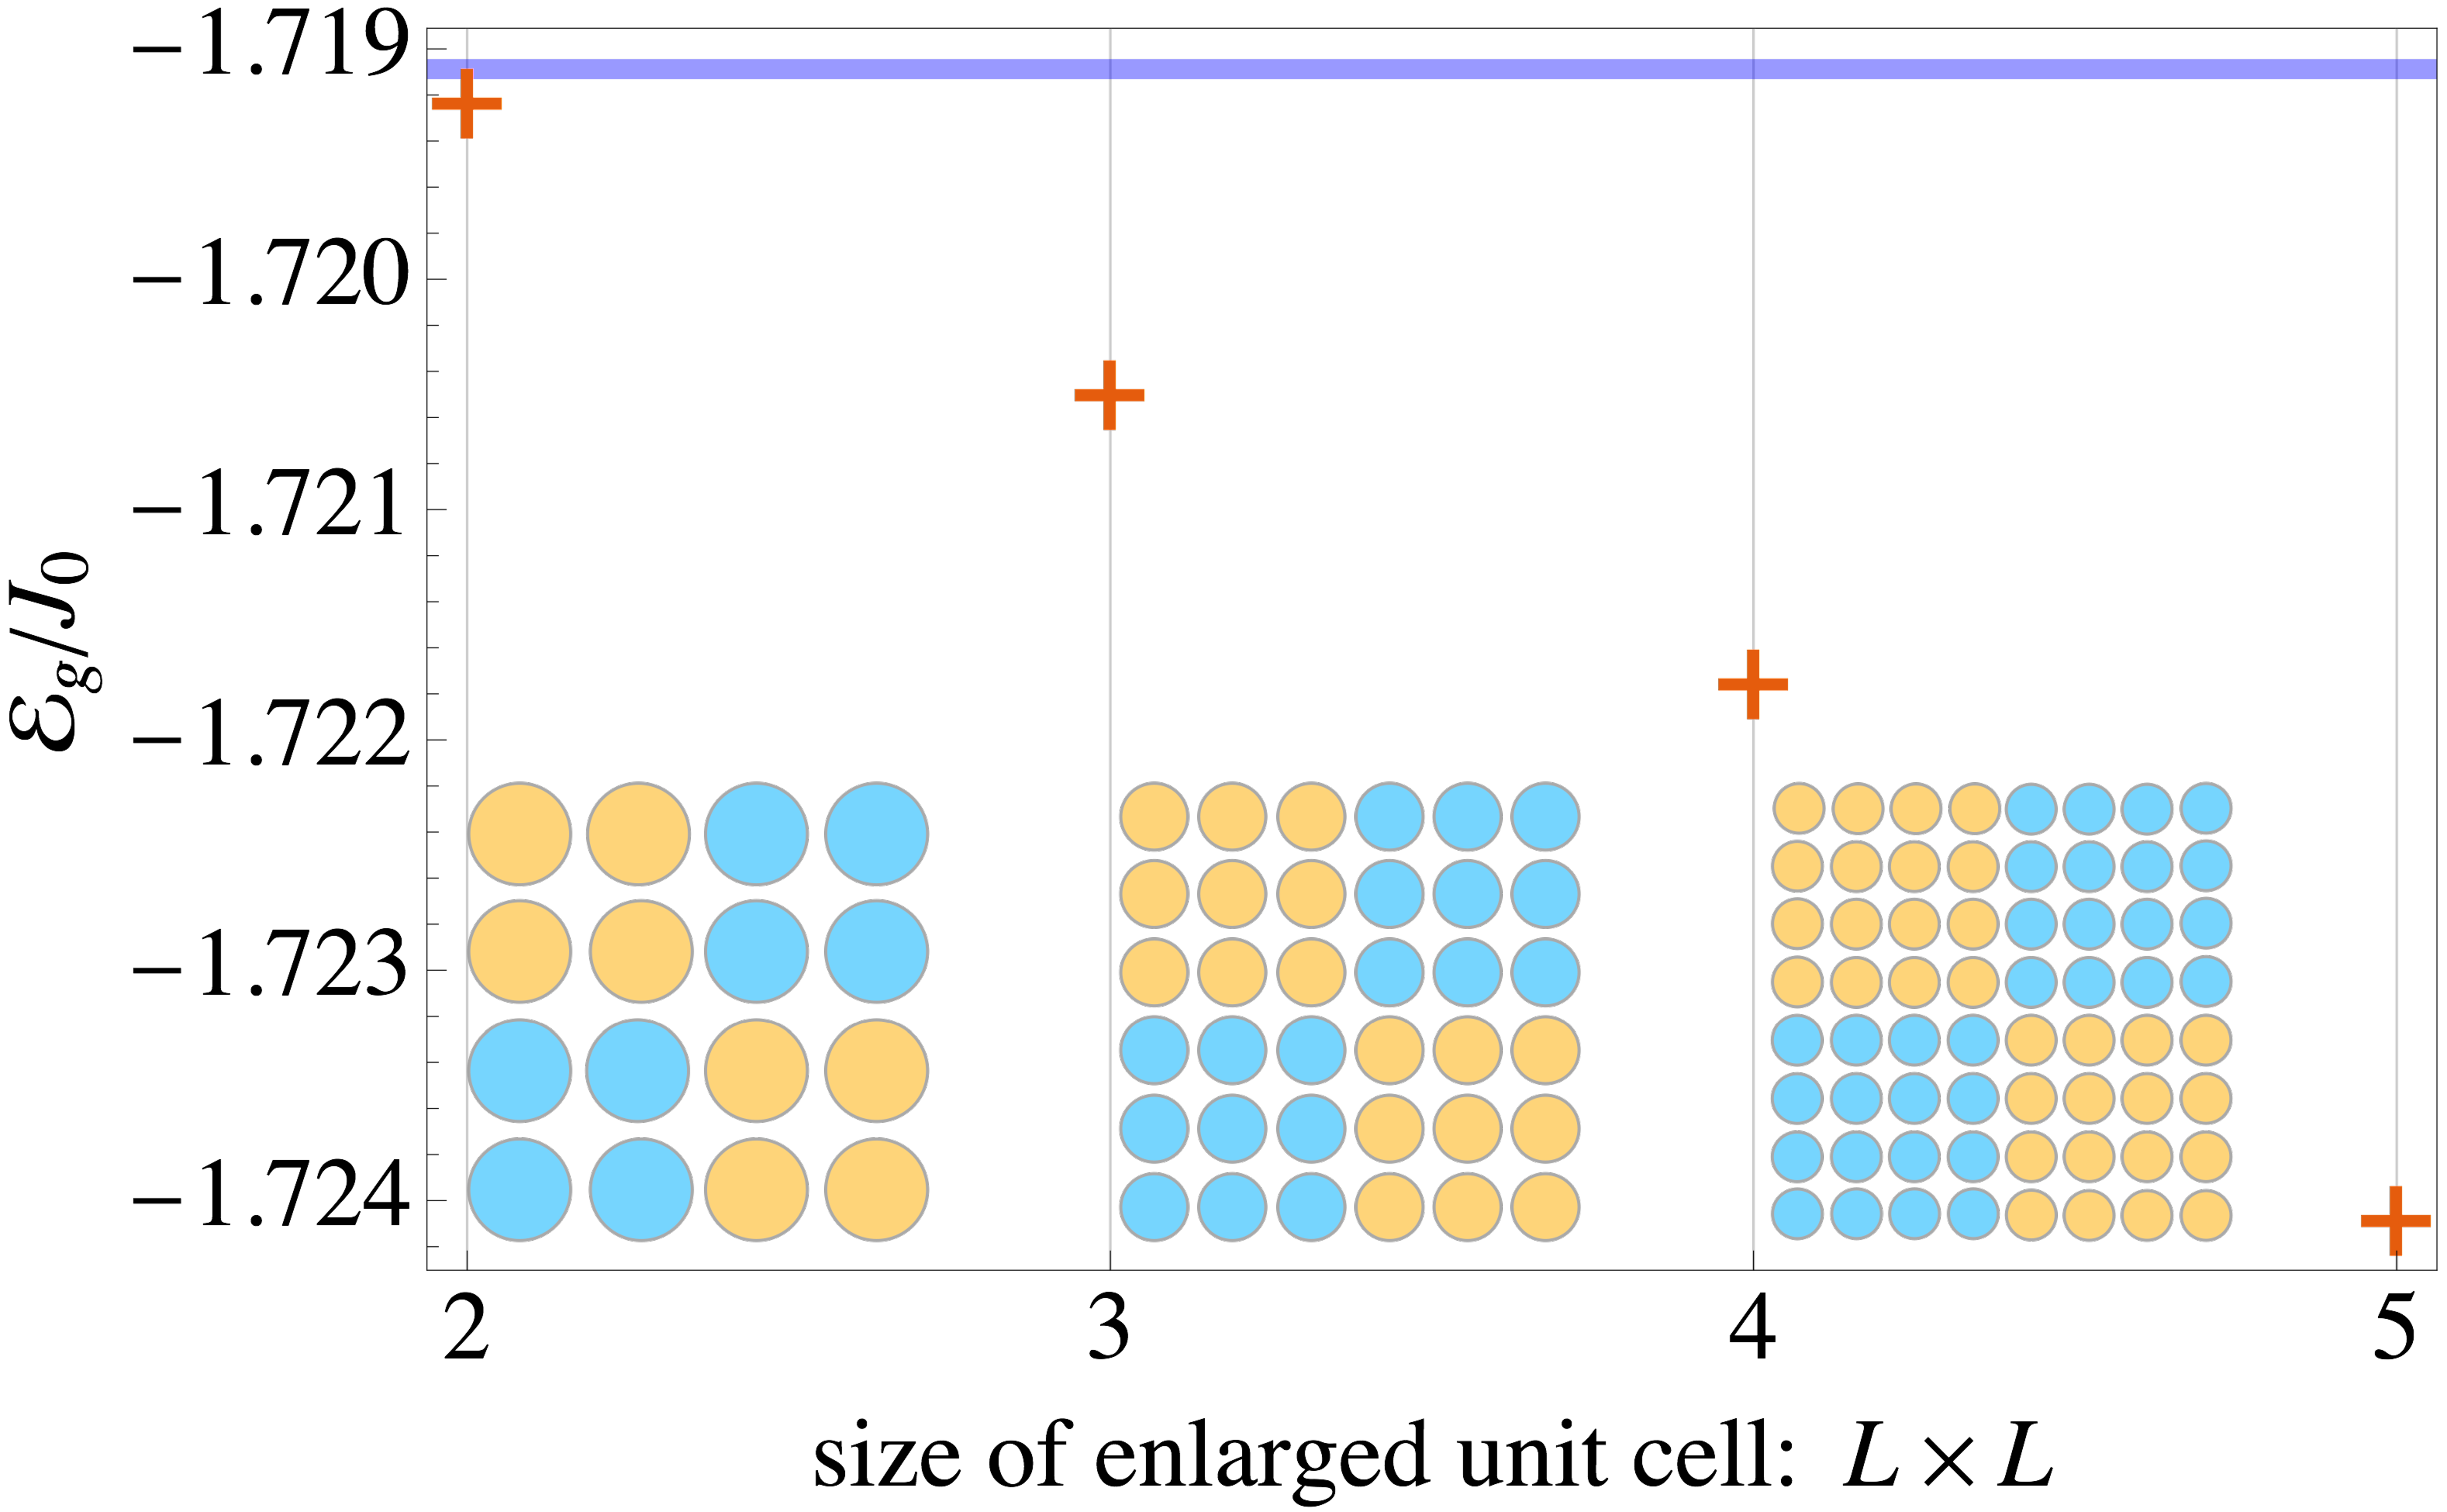
\includegraphics[width=.5\columnwidth]{figs/phase_separation.pdf}
\end{figure}
\end{block}
\end{frame}

\begin{frame}\frametitle{Correlated tunneling induced Ferro. Magn.}
\begin{block}{intra- vs. inter-}
\begin{minipage}{.3\columnwidth}
\begin{figure}
    \centering
    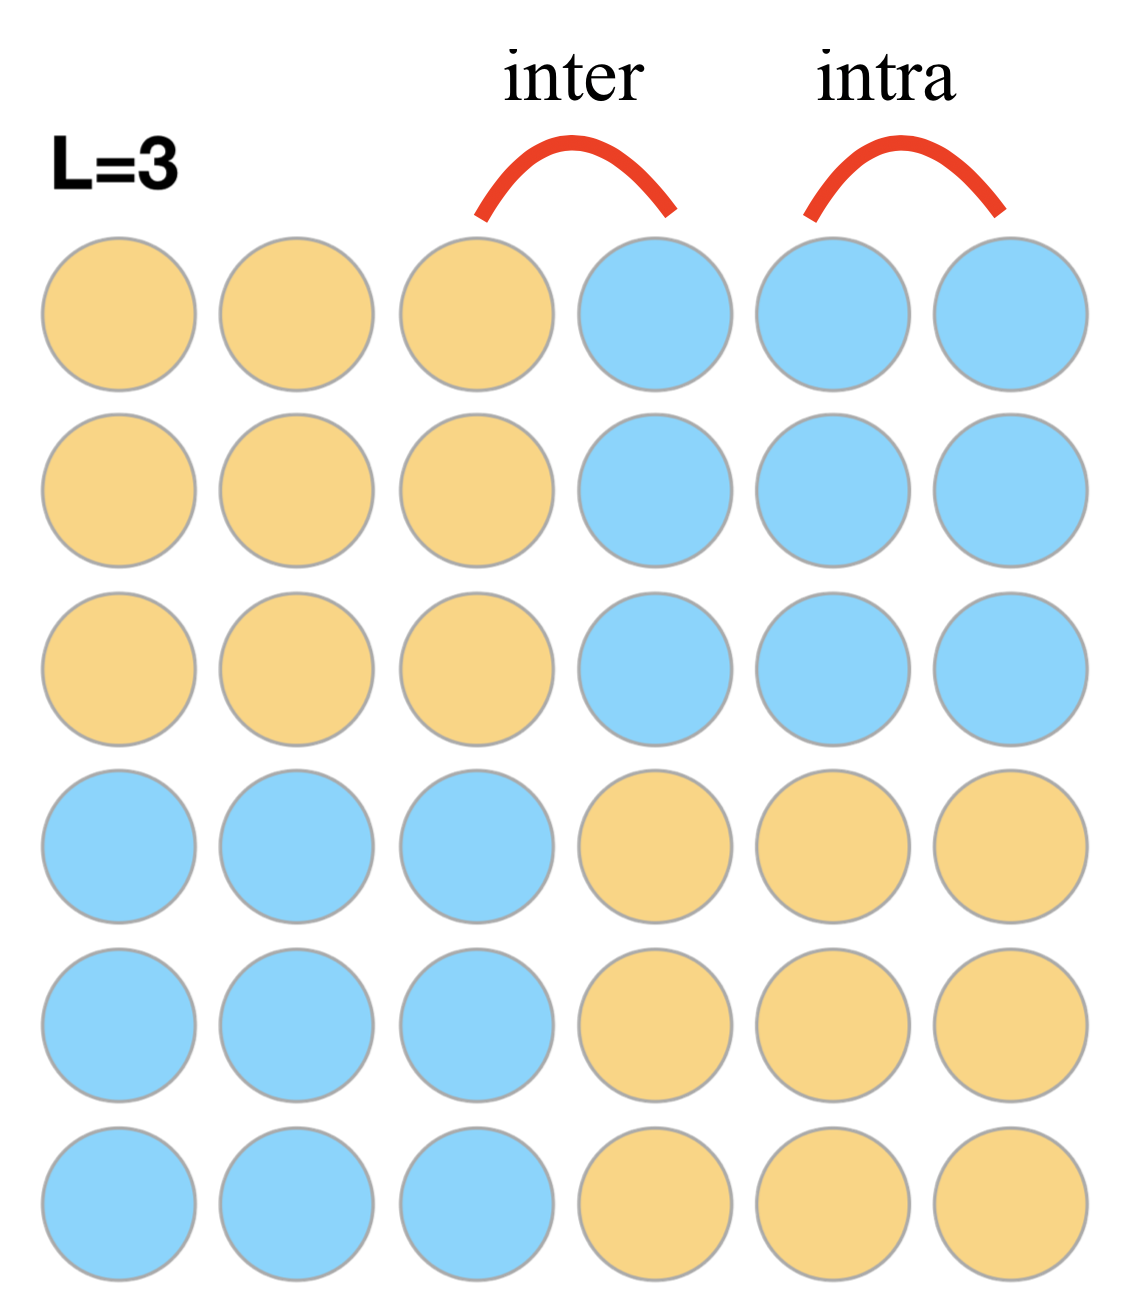
\includegraphics[width=.6\columnwidth]{figs/intra-inter.png}
\end{figure}
\end{minipage}
\begin{minipage}{.65\columnwidth}
\begin{align*}
	J^{\text{intra}}_{\text{eff},\sigma} &= 
        \frac{1}{2} \left(J_0[1+(c\mp s)^2]+J_1[1-(c\mp s)^2]\right), \\
	J^{\text{inter}}_{\text{eff},\sigma} &= 
        \frac{1}{2} \left(J_0[1-(c\mp s)^2]+J_1[1+(c\mp s)^2]\right),
\end{align*}
\end{minipage}
\end{block}
\pause
\vspace{-1ex}
\begin{block}{tunneling energy of no interaction}
\begin{figure}
    \centering
    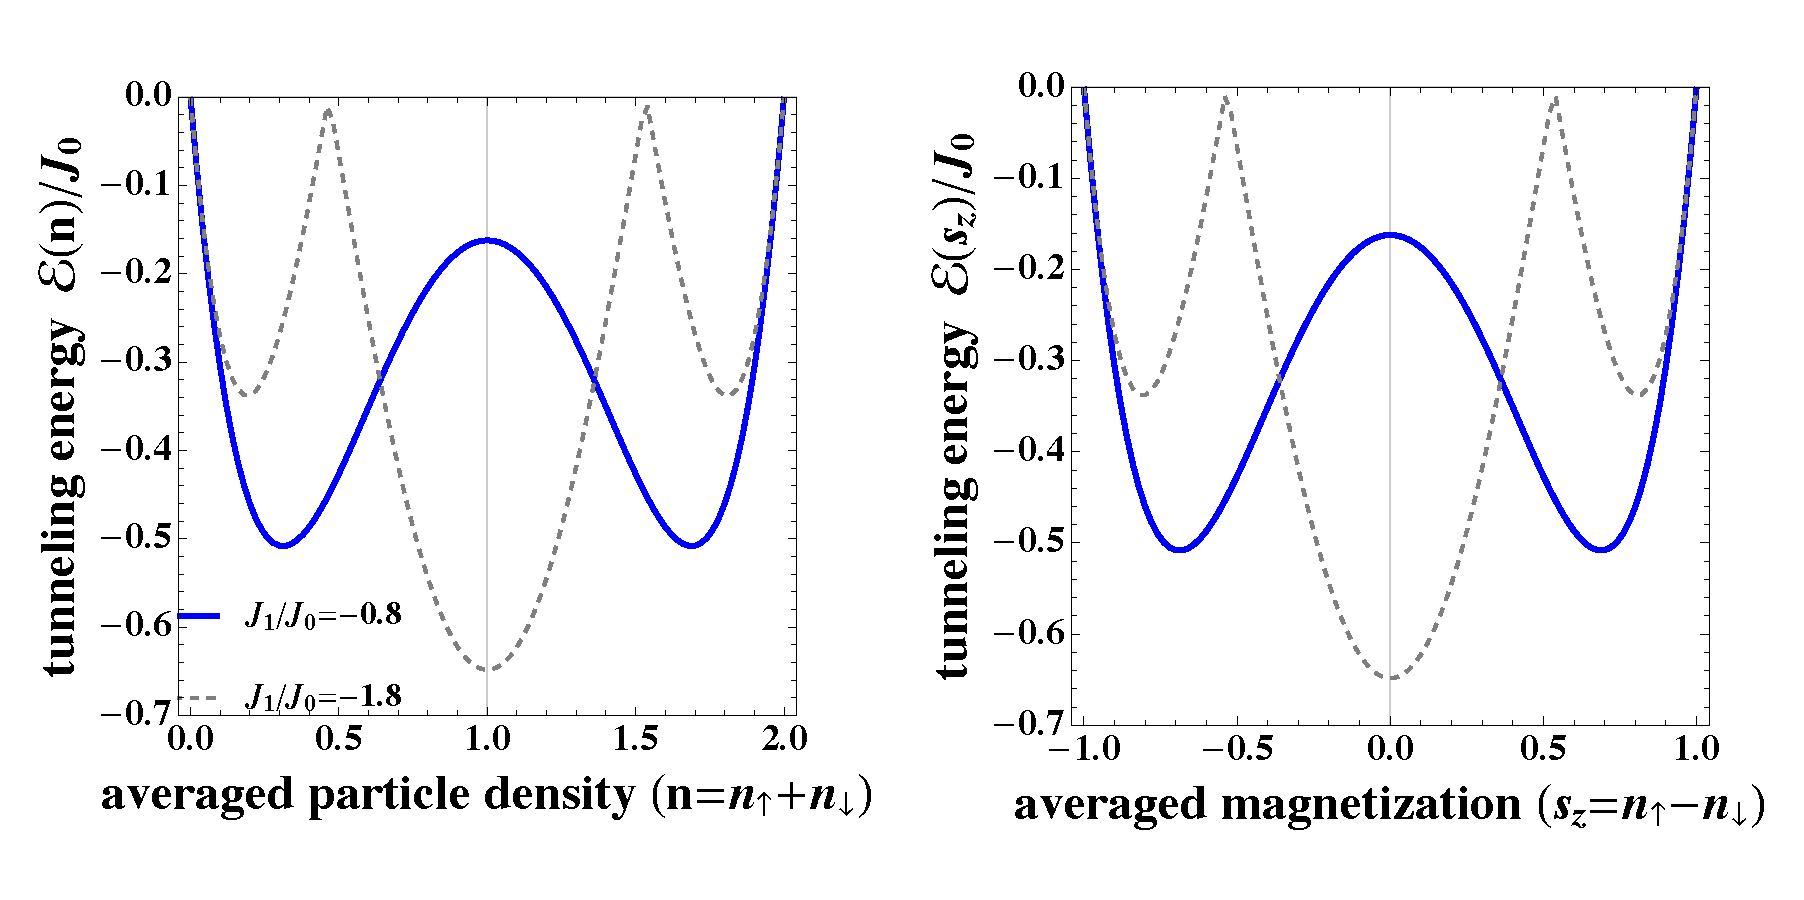
\includegraphics[width=0.6\columnwidth]{figs/kinetic_energy.pdf}
\end{figure}
\end{block}
\end{frame}


\section{Conclusion}
\begin{frame}\frametitle{Summary}
\begin{block}{Conclusion}
\begin{itemize}
\pause
\item Fermi Hubbard model on 2D square lattice with correlated hopping
\pause
\item Mean field phase diagram: CDW/P, SDW, co-existence
\pause
\item FM/PS phase
    \begin{itemize}
\pause
    \item at small $\tilde{U}$
\pause
    \item alternative machenism: induced by correlated hopping
    \end{itemize}
\pause
\item Expected to be verified by experiment.
\end{itemize}
\end{block}
\end{frame}


\section*{Acknowledgment}
\begin{frame}
\begin{block}{Acknowledgment}
\begin{figure}[!htb]
    \centering
    % 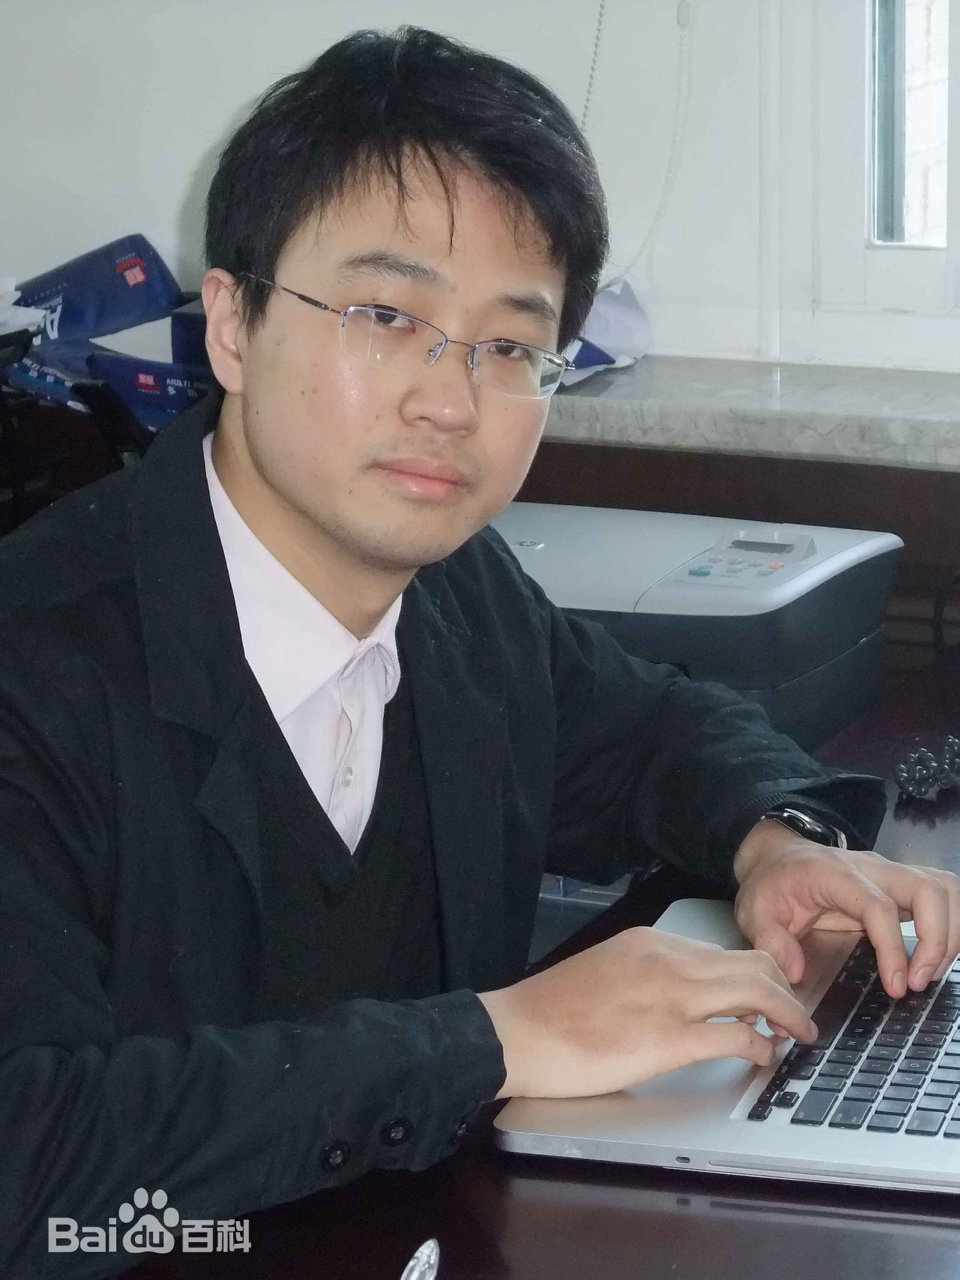
\includegraphics[width=0.4\columnwidth]{figs/huizhai.png}
    % 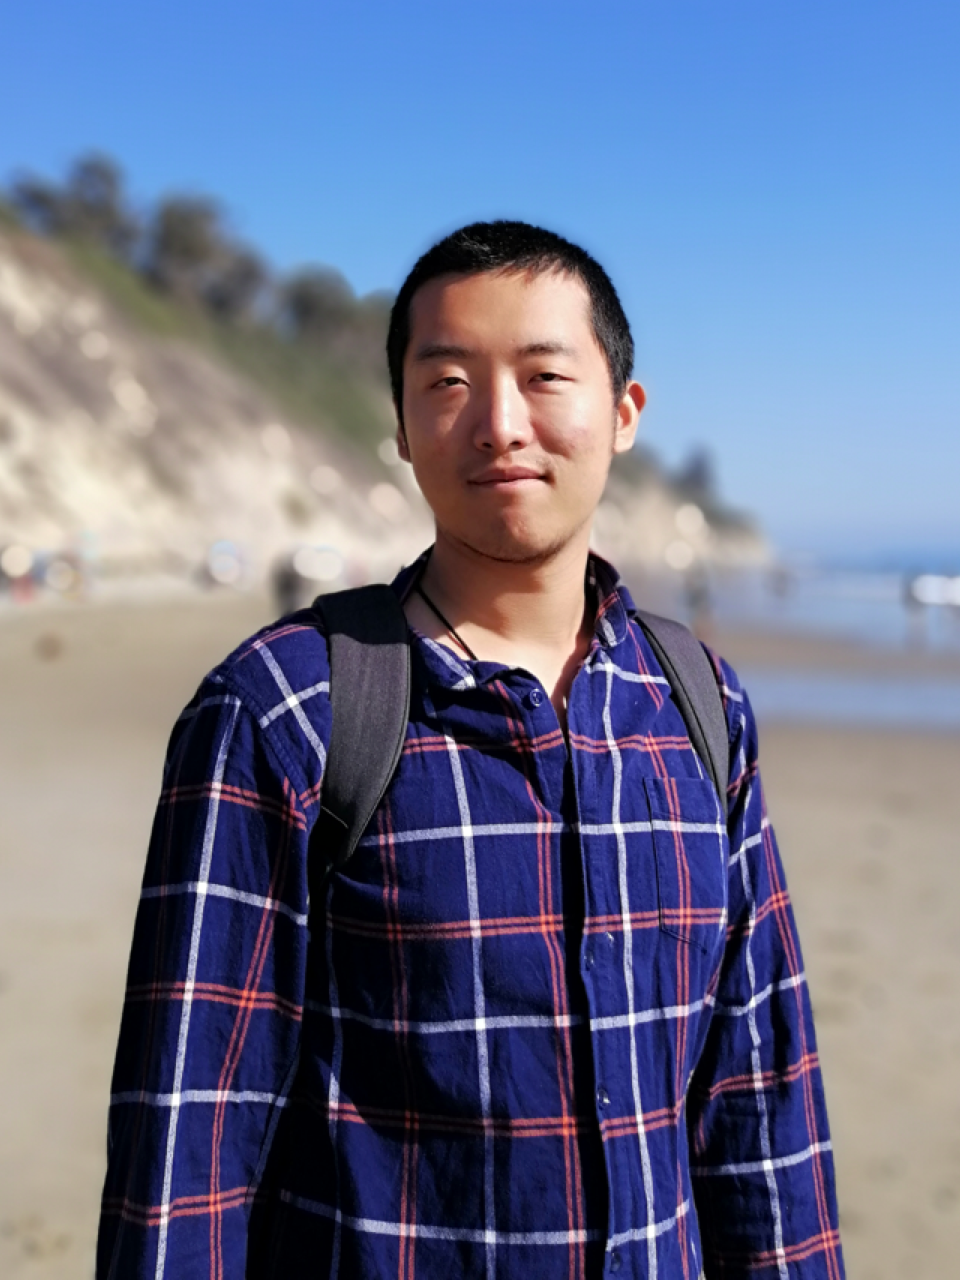
\includegraphics[width=0.4\columnwidth]{figs/pengfei}
    \subfloat[Pengfei Zhang]{
        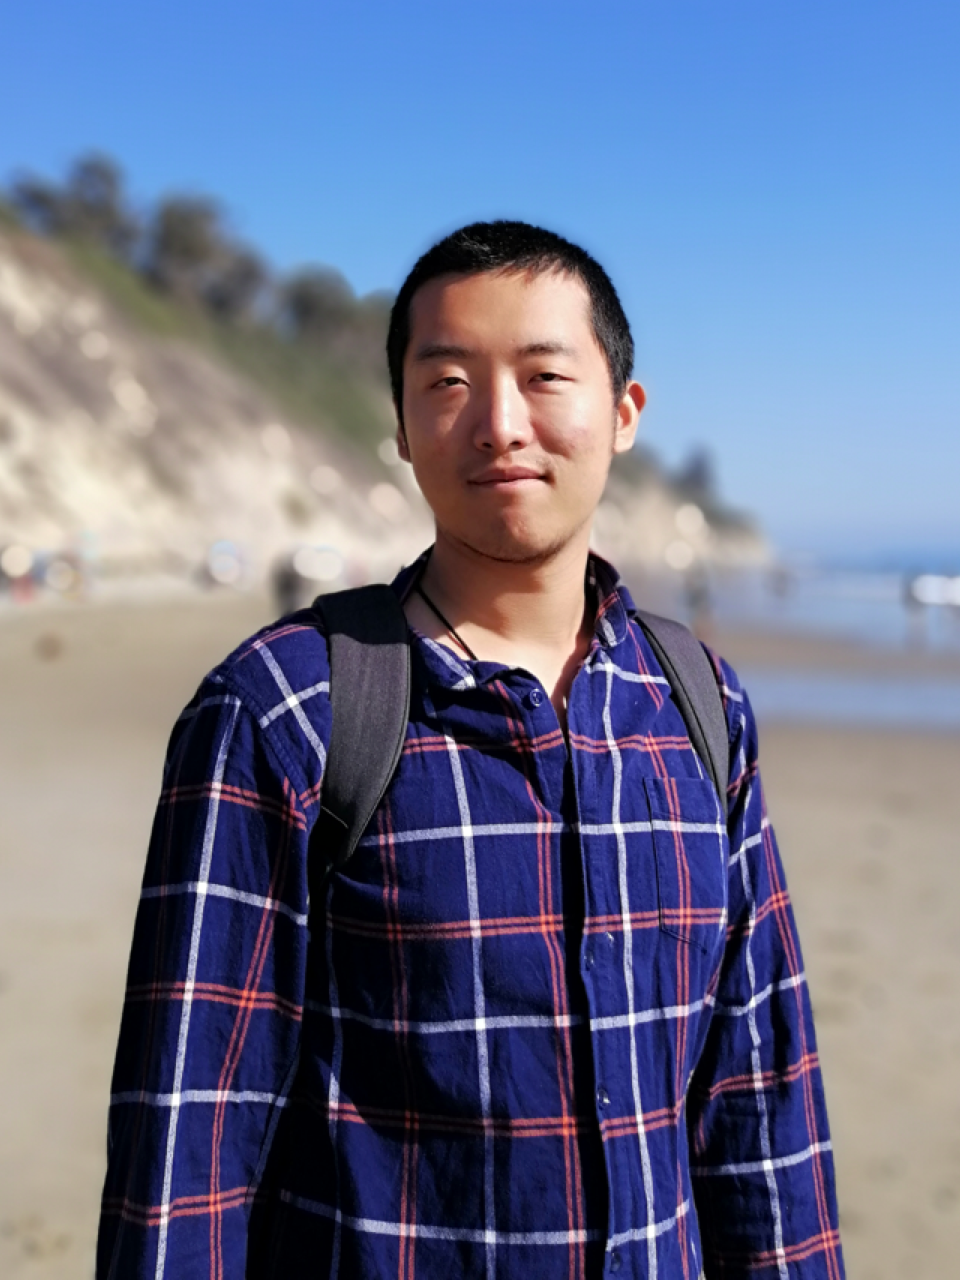
\includegraphics[width=.34\columnwidth]{figs/pengfei.png}
    }
    \subfloat[Prof. Hui Zhai]{
        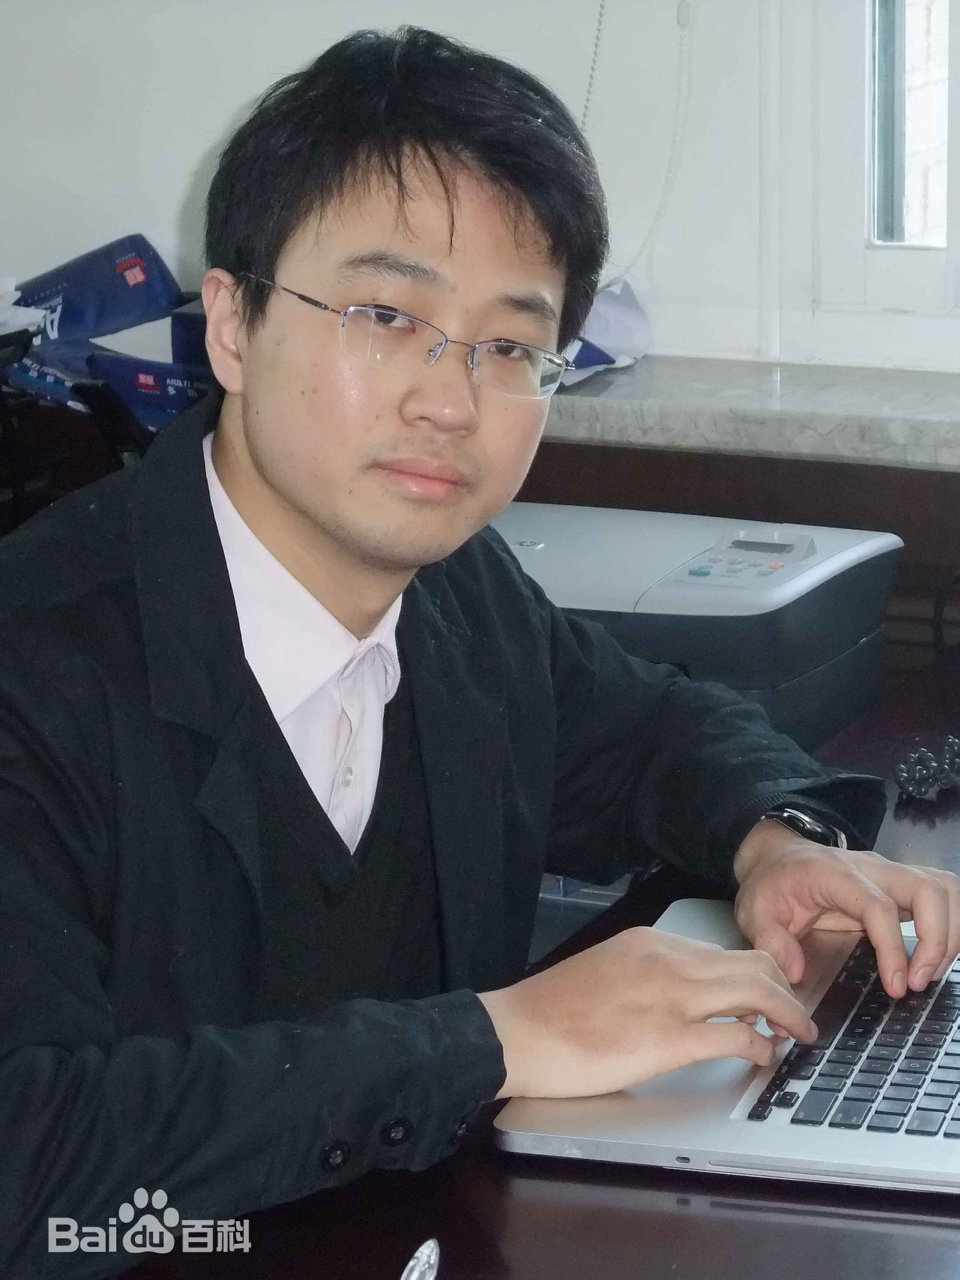
\includegraphics[width=.34\columnwidth]{figs/huizhai.png}
    }
\end{figure}
\end{block}
\end{frame}


\section*{End}
\begin{frame}
\centering
    \Huge
    Thank You!
\end{frame}


\end{document}
